%!TEX root = ../Thesis.tex
\label{chapter:data_collection}
\paragraph{}
In this chapter, we will discuss the method and procedure used to collect physiological data of the subjects. We will discuss the available options for collecting the physiological signals required for our analysis and why we chose BITalino (r)evolution Plugged Kit BT. In the latter part of the chapter, we take a look at some of the challenges faced while recording the physiological signals and how we overcome those challenges. We conclude the chapter by discussing the experimental setup for the study.
\section{Device Selection}
As we have discussed in Chapter \ref{chapter:Terminology}, the significant physiological signals we wished to collect for the study were Electrocardiogram (ECG) and Electrodermal activity (EDA). Using currently commercially available fitness trackers like Apple Watch, Garmin Vivoactive, etc. would not suffice our experimental requirements. The aforementioned devices are not yet capable of recording high quality ECG and EDA signals. Thus, we preferred to use a biosignal acquisition device which can record high quality \textbf{raw} physiological signals. We found BITalino (r)evolution Plugged Kit BT to be the best fit for our study. There were two main reasons for choosing BITalino (r)evolution Plugged Kit BT. First, we were able to get high-resolution physiological signals (at 100Hz) and second, we presume that in future the fitness trackers would be sophisticated enough to record the signals at a higher resolution.
\begin{figure}
\centering
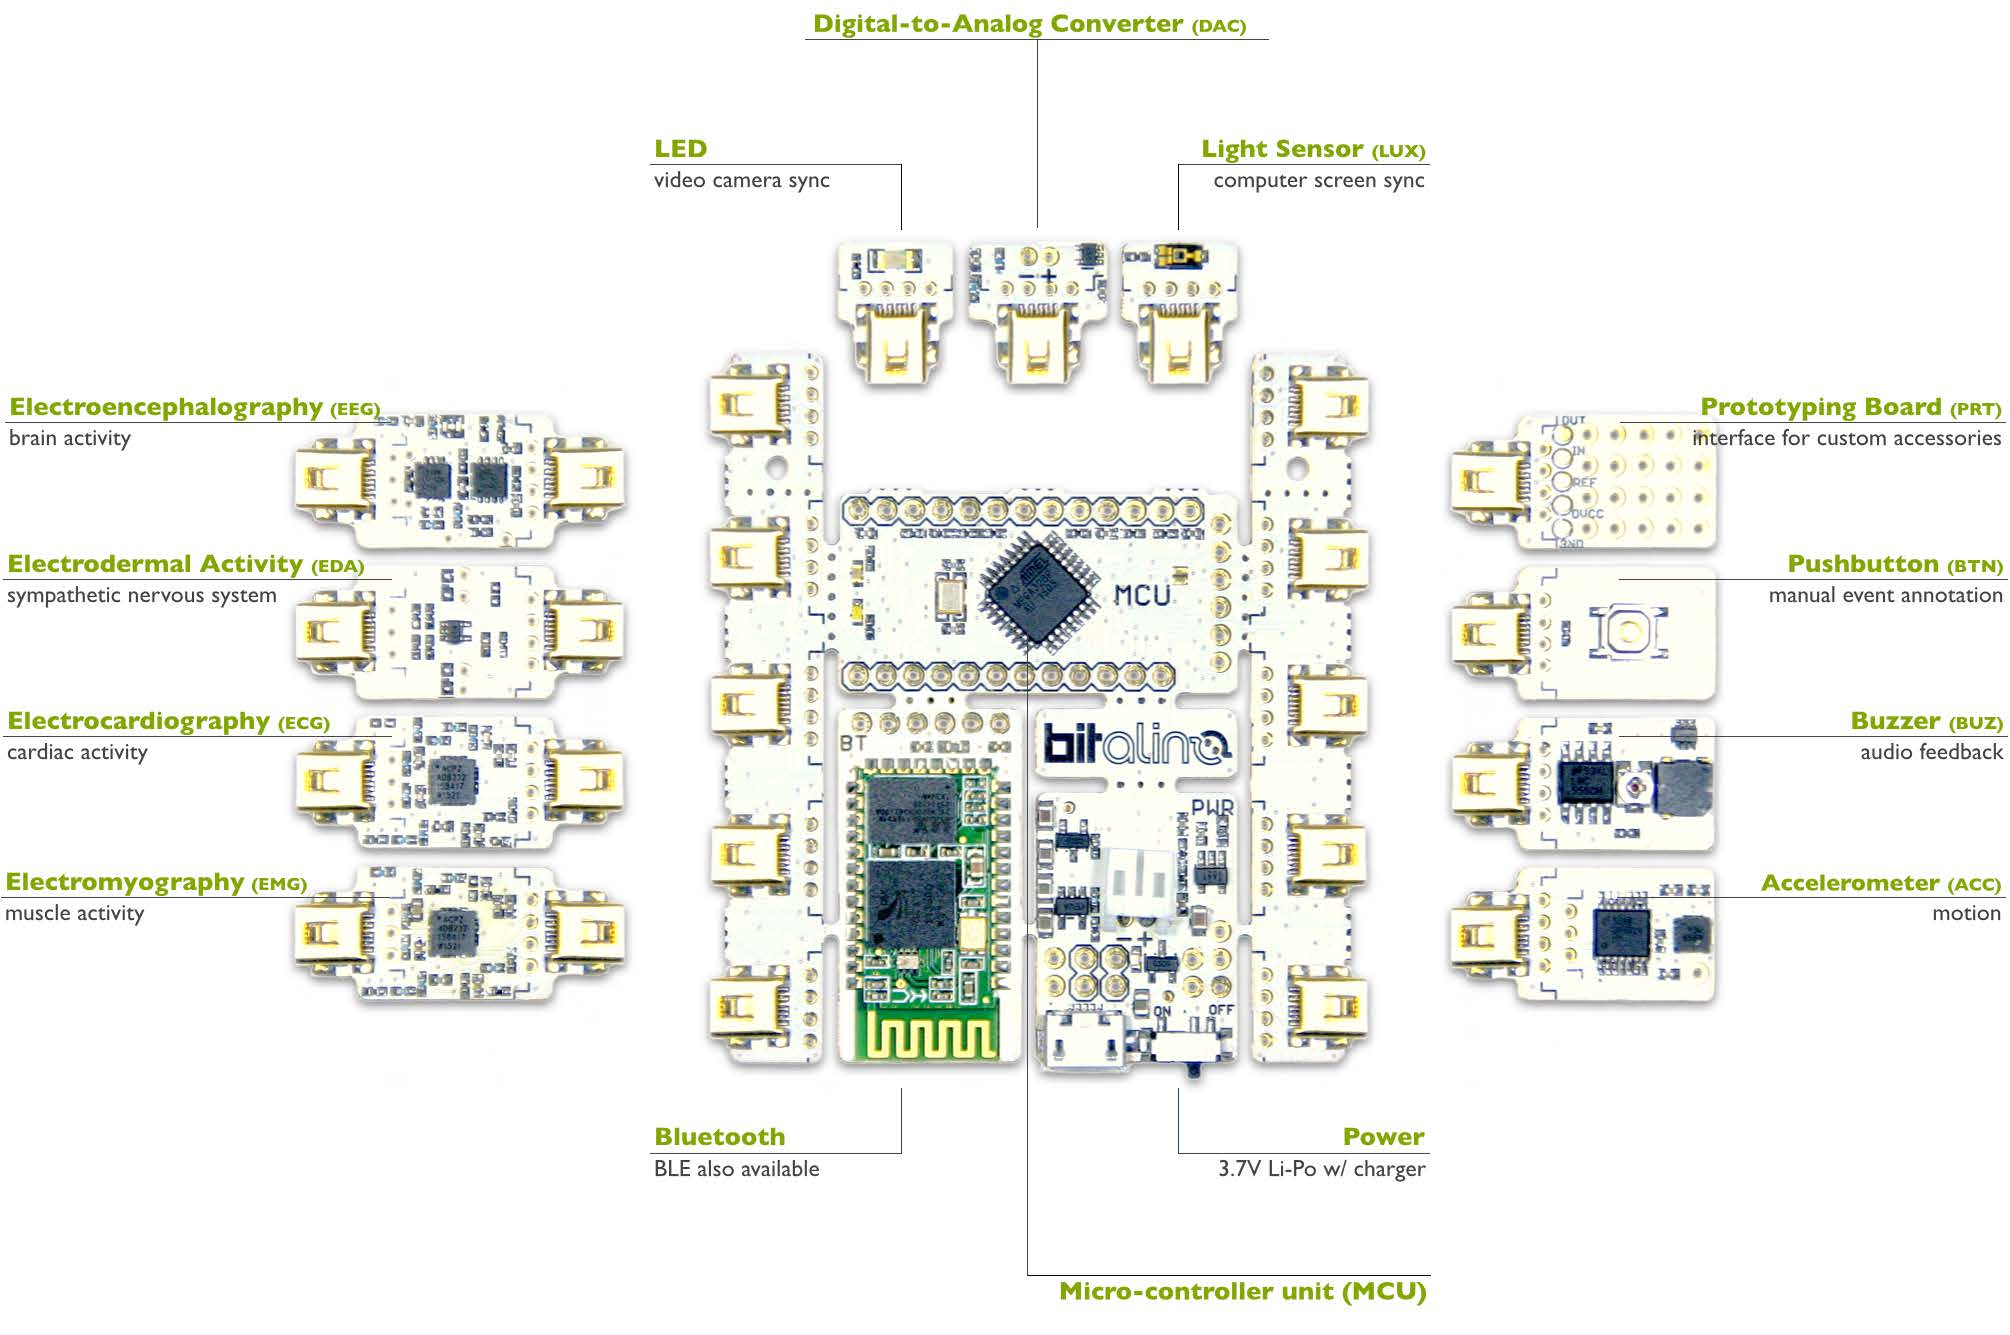
\includegraphics[width=140mm]{Figures/bitalino.jpg}
\caption{BITalino (r)evolution Plugged Kit BT \cite{bitalino_datasheet}.}
\label{fig:bitalino}
\end{figure}
\paragraph{BITalino (r)evolution Plugged Kit BT} BITalino is an all-in-one board designed for biosignal acquisition. The main board connects with sensors, which are separate components using UC-E6 socket as shown in Figure \ref{fig:bitalino} \cite{bitalino_datasheet}. Using BITalino over other biosignal acquisition devices or fitness trackers are discussed in the following subsection,

\subsection{Medical Expertise} Most medical grade devices require technical expertise and knowledge of anatomy to configure and operate. Moreover, high-end medical devices are expensive and time-consuming to operate. Thus, we decided on to highly versatile and easy to operate framework, BITalino.

\subsection{Quality of Data} When it comes to biosignal acquisition there are strict terms in regards to signal parameters. While converting from analog to digital signals, the instrumentation is required to be designed with high Signal to Noise Ratio (SNR) and accurate sampling rate. BITalino enables high accuracy conversion of analog to digital signals \cite{guerreiro_performance_2014}.

\subsection{Availability of data} BITalino provides a Biotech Application Programming Interface (API) which allows incorporating BITalino into custom made application software \cite{noauthor_biotech_nodate}. This allowed us to design application software suited to our data acquisition requirements. We designed an application that is capable of acquiring data from six BITalino devices over the Bluetooth. Since each device has four ports (see section \ref{design_principles}), we were able to record ECG and EDA data from 12 subjects simultaneously. The details of the application are discussed in Section \ref{sec:custom_int}. The Application Programming Interface (API) also allows time synchronization between multiple devices which will be discussed in section \ref{sec:time_sync}.

\section{Anatomy of BITalino}
\subsection{Design Principles}
\label{design_principles}
BITalino is a 100x65x6mm chip onboard device that integrates multiple plug and play sensors to measure bio-electrical and biomechanical data. The digital back-end is supported by a control block based on ATmega328P micro-controller, and a communication block that uses a Class II Bluetooth v2.0 module for wireless data transfer to a base station (example. Computer, Mobile Phone etc) \cite{silva_bitalino:_2014}.

\paragraph{} BITalino is capable of recording at 1, 10, 100 or 1000 Hz frequency. It has four 10-bit analog ports and two 6-bit analog ports which can be utilized to connect to plug and play sensors to record physiological signals of the subjects. The detailed specification of the device is listed in table \ref{tab:bitalino_specification} \cite{bitalino_datasheet}.

\begin{center}
\begin{tabular}{ |c|c| }
\hline
Sampling Rate & 1,10,100 or 1000 Hz \\
\hline
Analog Ports & 4 in (10-bit) + 2 in (6-bit) \\
\hline
Digital Ports & 2 in (1-bit) + 2 out (1-bit) \\
\hline
Bluetooth Range & up to approx. 10m (in line of sight) \\
\hline
Sensors & EMG; ECG; EDA; EEG; ACC; LUX; BTN \\
\hline
Actuators & LED; BUZ \\
\hline
Size & 100x65x6mm \\
\hline
Battery & 500mA 3.7V LiPo (rechargable) \\
\hline
Consumption & approx. 64mA \\
\hline
Accessories & 1x3-lead cable; 1x2-lead cable. \\
\hline
\end{tabular}
\captionof{table}{Specification of BITalino (r)evolution Plugged Kit \cite{bitalino_datasheet}.}
\label{tab:bitalino_specification}
\end{center}

\subsection{ECG Sensor}
The ECG sensor of BITalino operates in the range of -1.5mV to +1.5mV and bandwidth between 0.5-40Hz. The sensor has a gain of 1100 and input impedance of 7.5GOhms \cite{ecg_datasheet}. The ECG Sensor is connected to the three-lead electrode, two of which are placed on the left and right under the collarbone and one is placed on the right of belly acting as the ground. The electrodes follow the Einthoven's triangle as discussed in section \ref{sec:einthoven}. The visualization of the lead placement is shown in Figure \ref{fig:ecg_lead_placement}
\begin{figure}
\centering
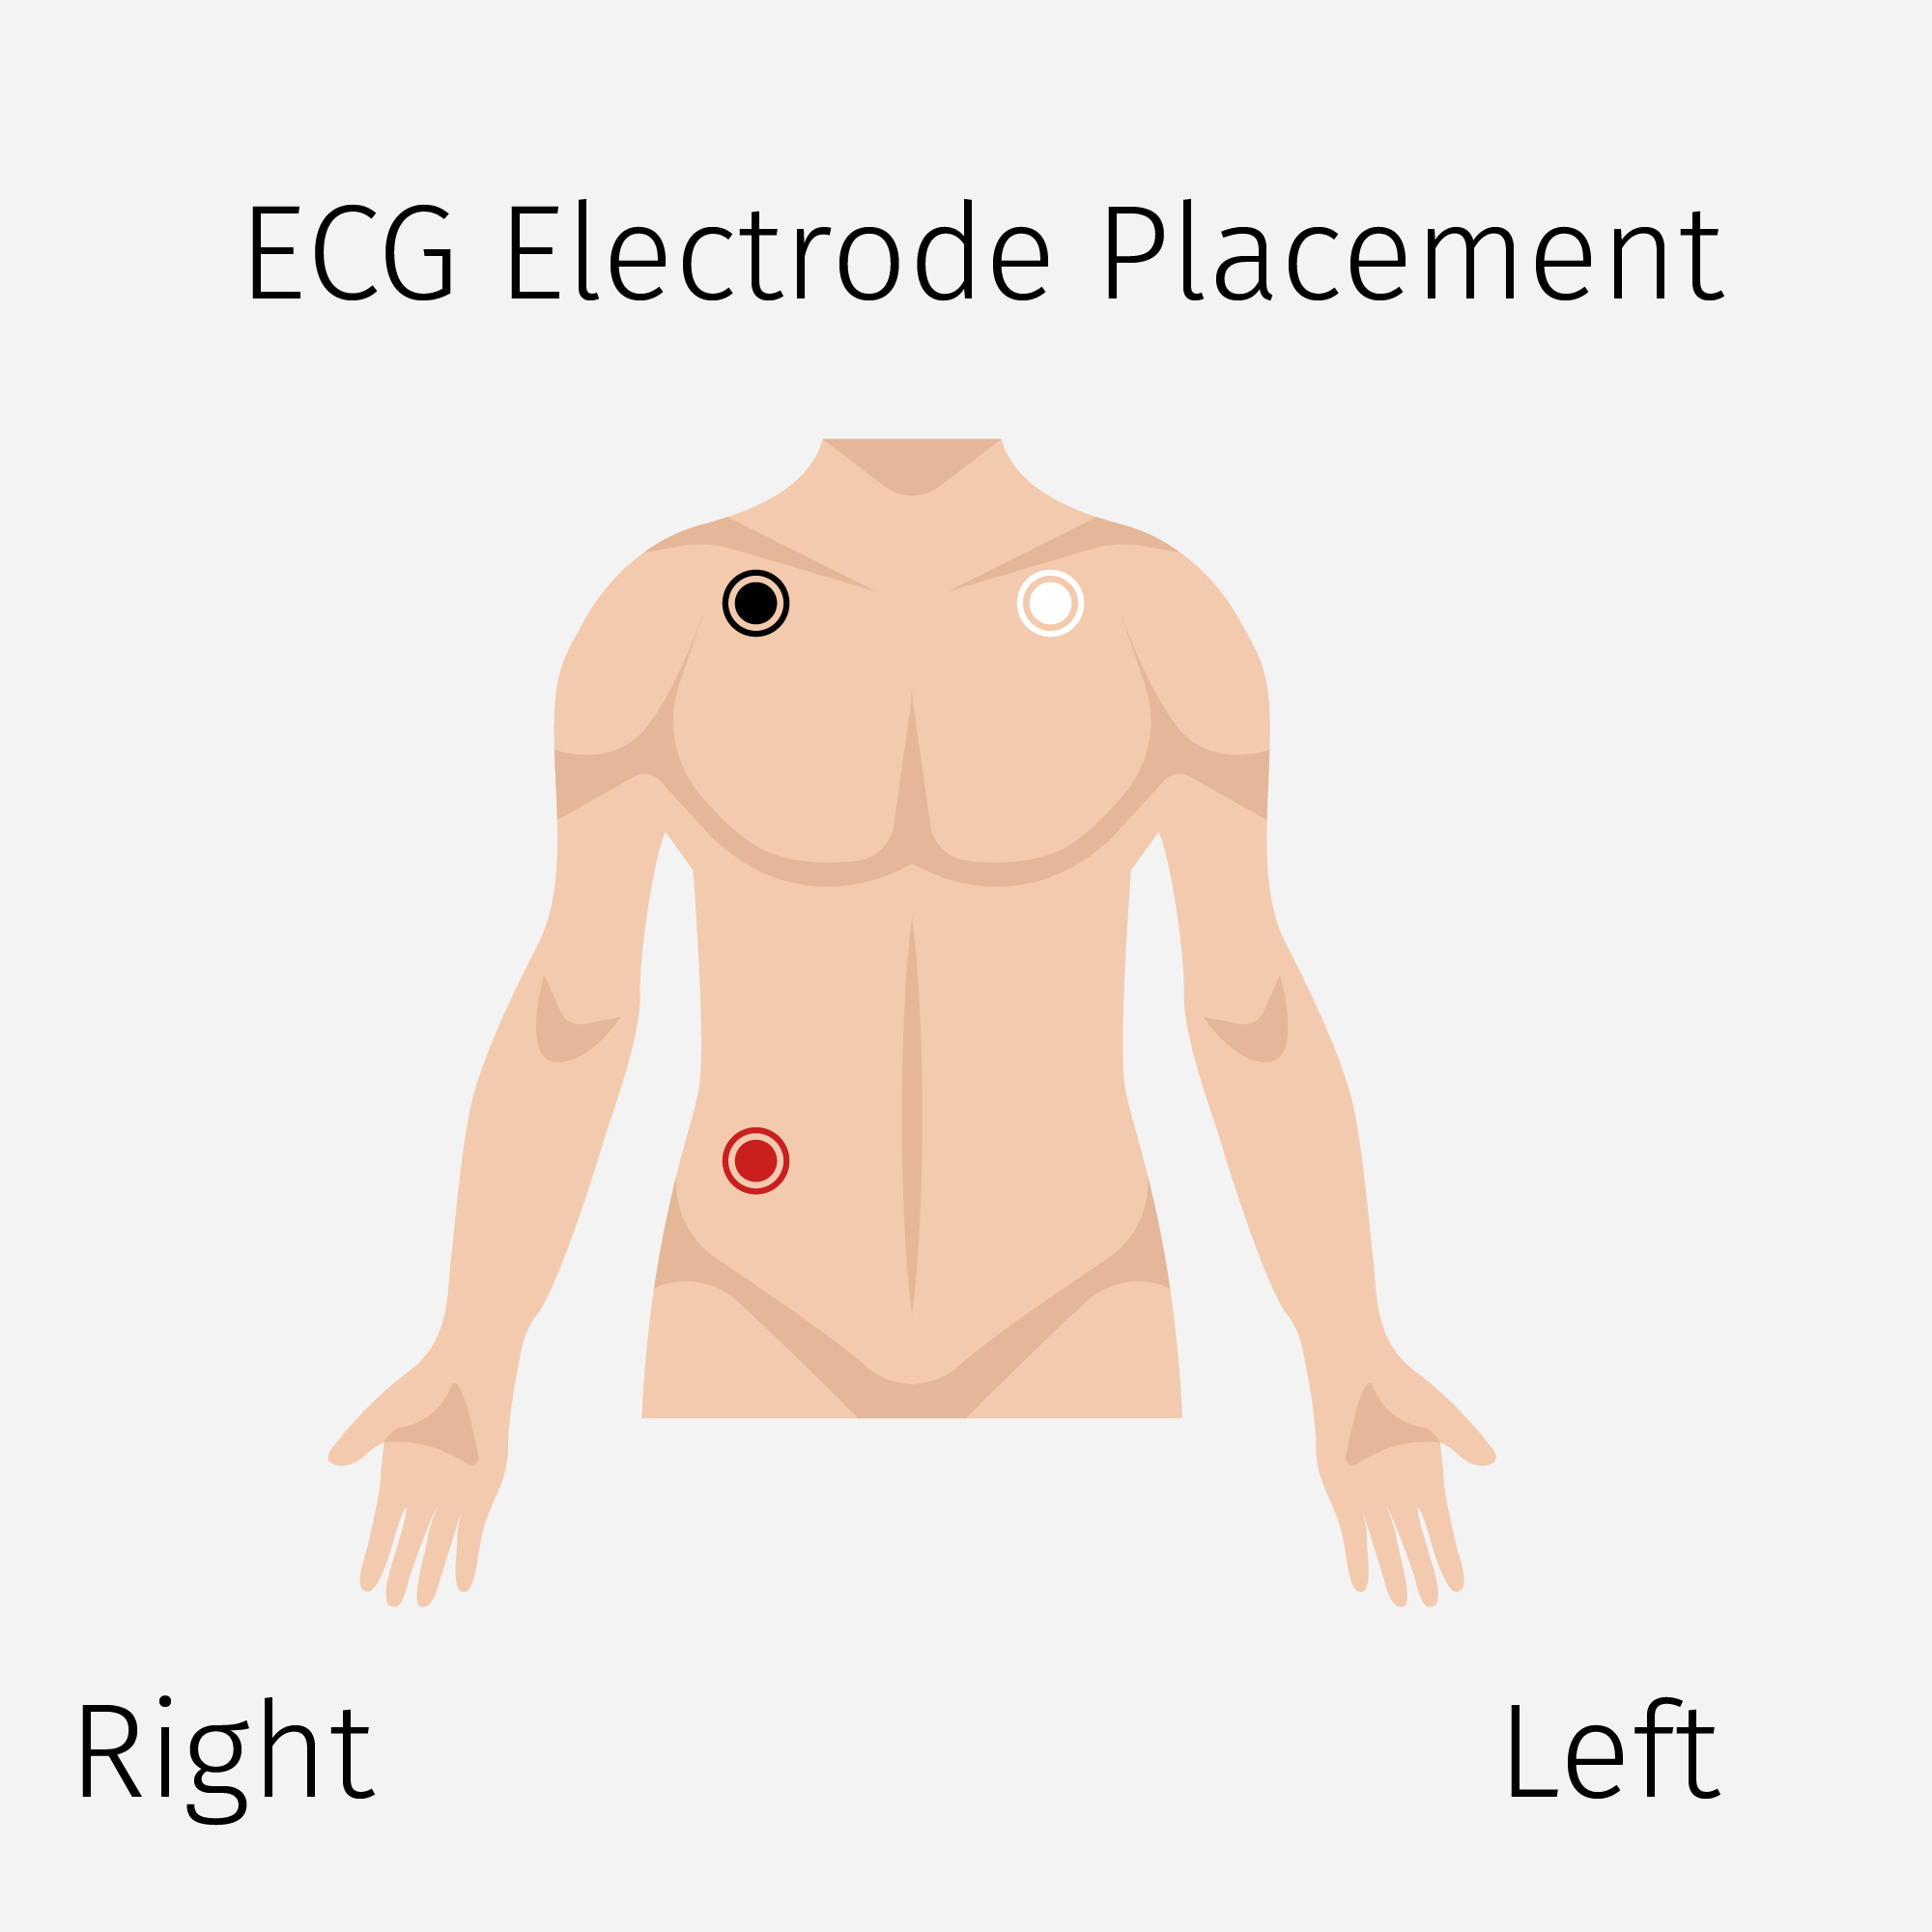
\includegraphics[width=100mm]{ECG.jpg}
\caption{ECG Lead placement.}
\label{fig:ecg_lead_placement}
\end{figure}
\subsection{EDA Sensor}
\label{sec:eda_sensor}
The EDA sensor of BITalino operates between 1.8-5.5V with a bandwidth between 0-2.8Hz. The EDA sensor is designed to record the EDA in the range between 0-25 $\mu$S with an input voltage of 3.3V \cite{eda_datasheet}. The EDA sensor is connected to a two-lead electrode which is placed on the tip or center of the index and middle finger of the subjects. The visualization of the lead placement is shown in Figure \ref{fig:eda_lead_placement}. We choose to place the EDA electrode on tip of the finger (Position 2) instead of middle part of the finger (Position 1) as discussed in Section \ref{sec:electrode_placement}. This was because many subjects that we tested with showed a lower sweat secretion resulting in very low EDA. Meanwhile, a select number of subjects registered EDA over threshold of the device due to high sweating. We moved the electrodes to middle part of finger for such subject. 
\begin{figure}
\centering
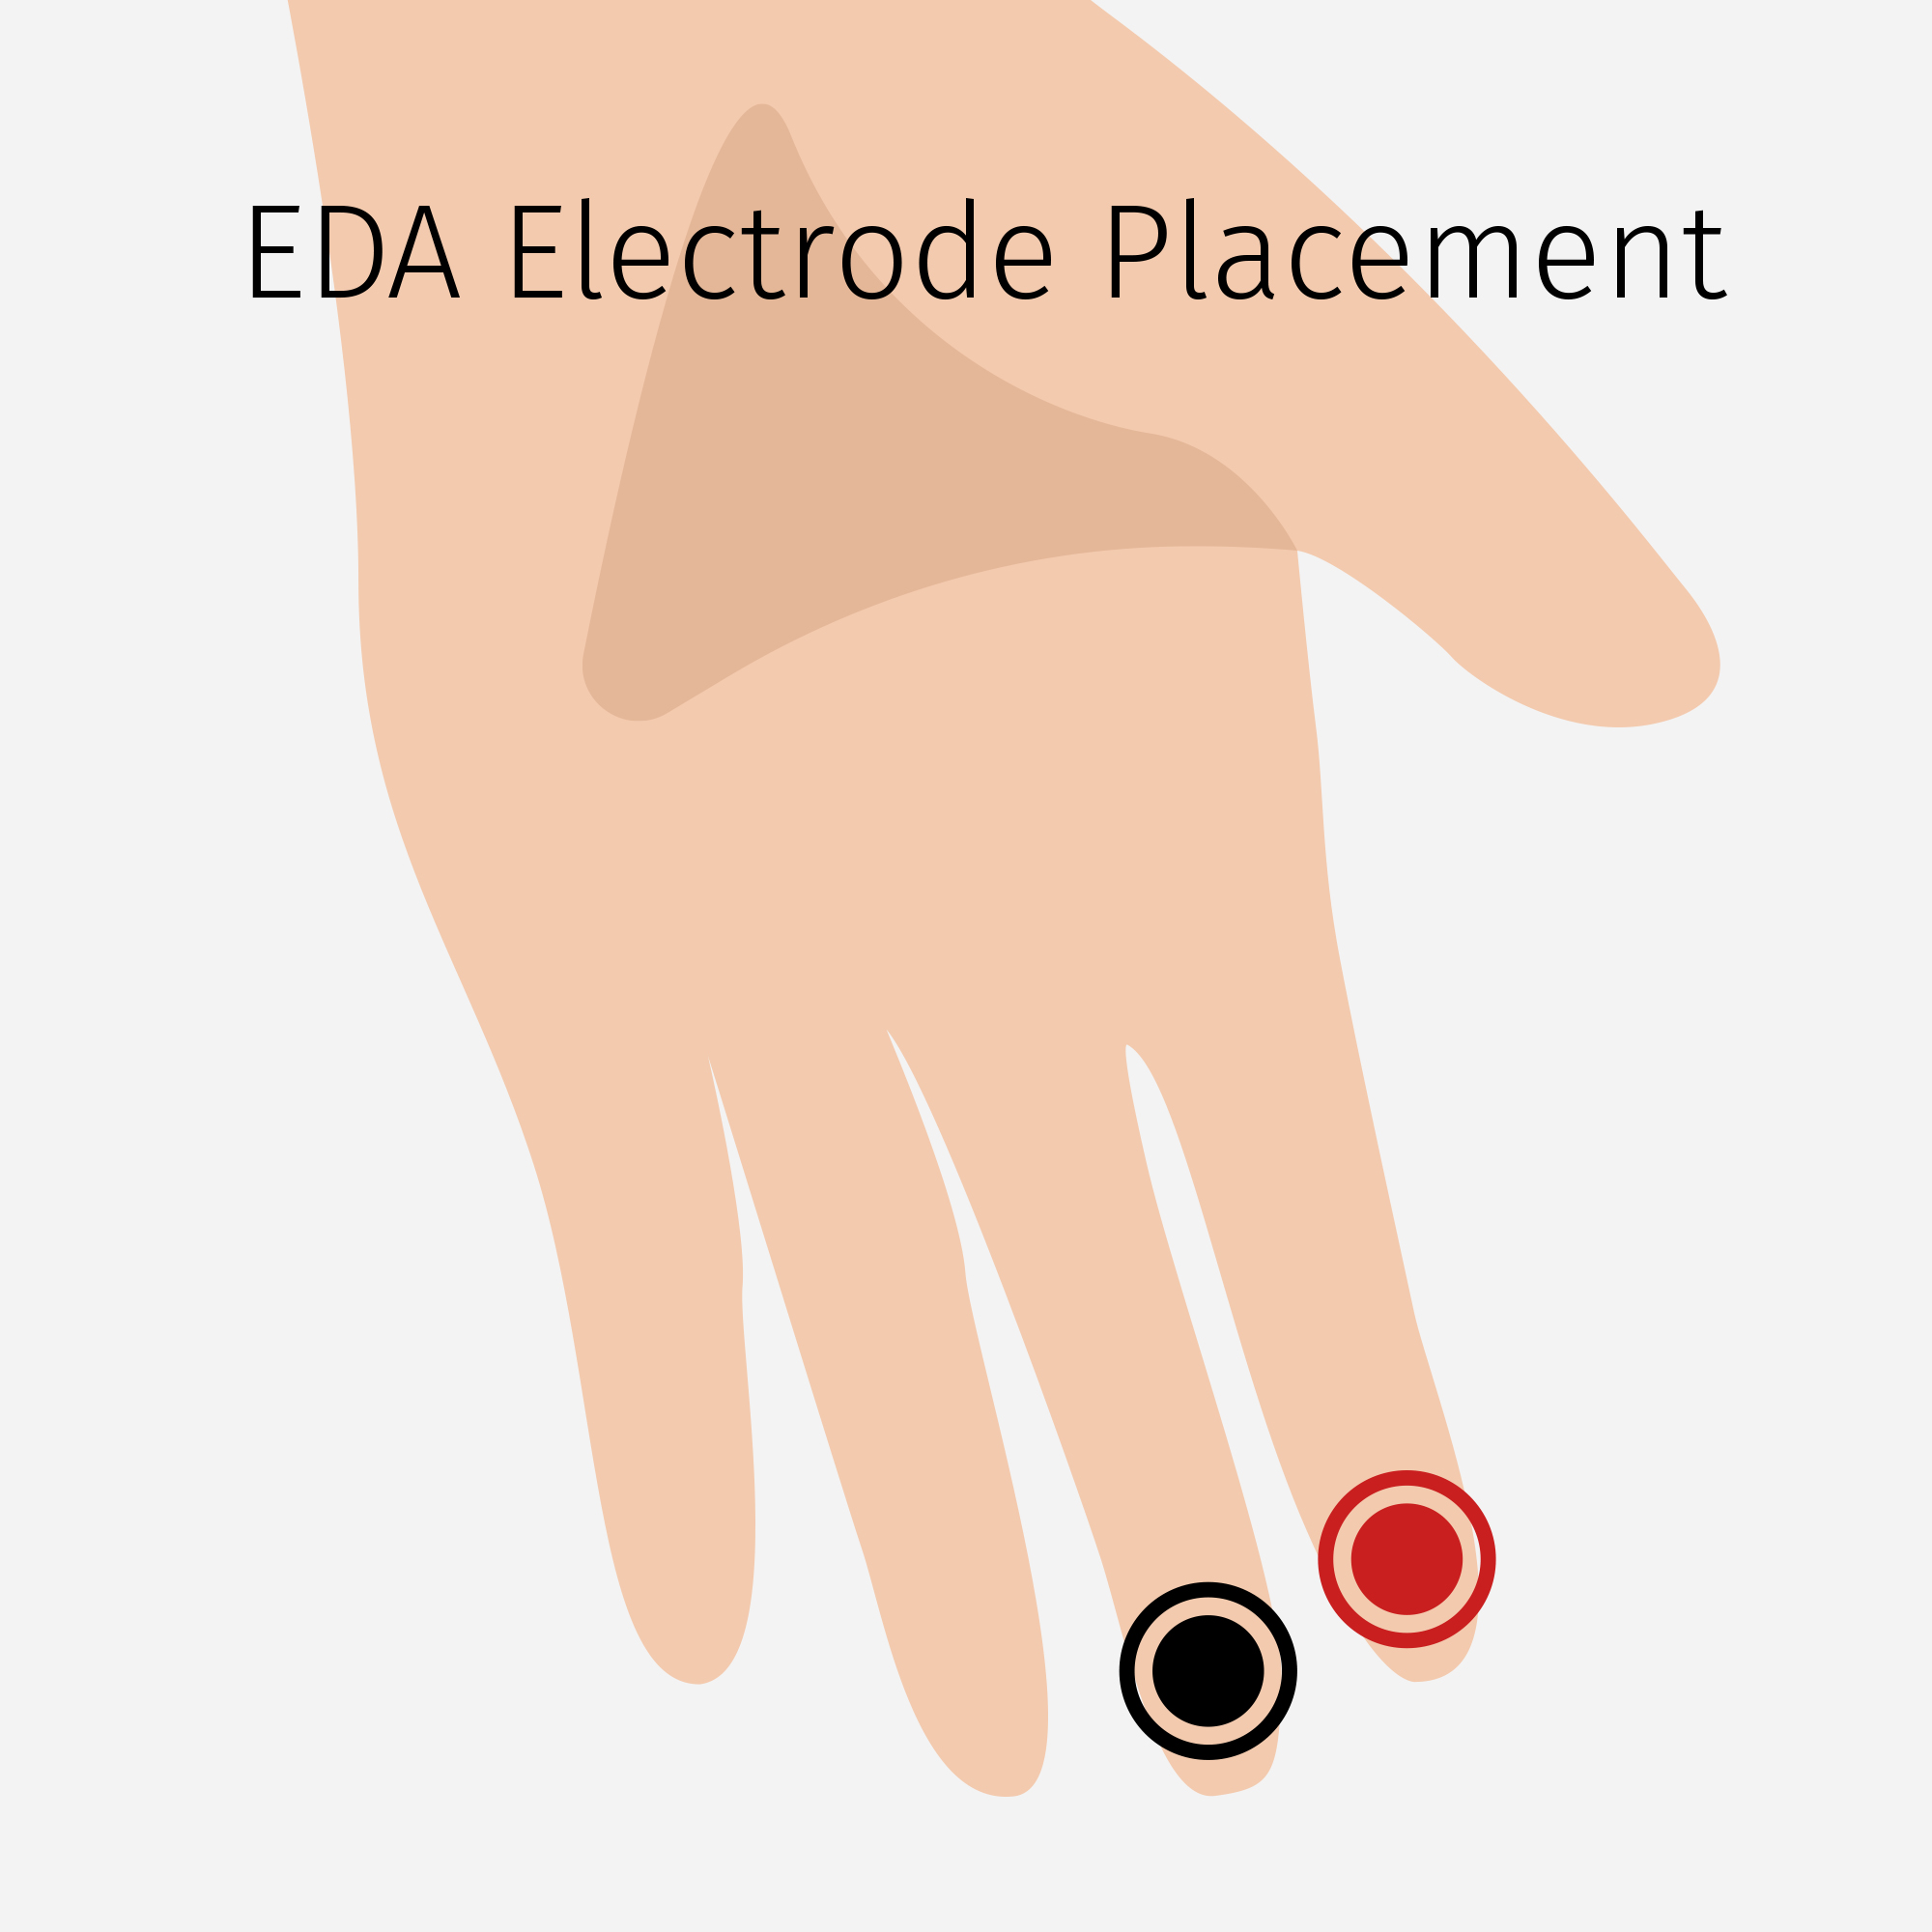
\includegraphics[width=100mm]{EDA.jpg}
\caption{EDA Lead placement.}
\label{fig:eda_lead_placement}
\end{figure}

\section{BITalino Configuration}
We set on to measure ECG and EDA of the subjects. Hence, we took advantage of ECG and EDA sensors of the BITalino. The sensors were then connected to two of four 10-bit analog BITalino’s analog ports. The leads of the electrodes were then connected to the subject. Since we wished to collect data from multiple subjects two subjects were connected to each BITalino device. We did not utilize the other two 6-bit analog ports. 
\paragraph{}
To further increase the number of subjects per session we utilized multiple BITalino devices. Having multiple devices connected and being recorded from simultaneously, posed a challenge of synchronizing the devices. Time synchronization of multiple devices is discussed in Section \ref{sec:time_sync}.
\paragraph{}
To make sure that we had the data required is time synchronized and annotated with the correct tags, we developed a custom application utilizing the BITalino API. The details of which are discussed in section \ref{sec:custom_int}.
\paragraph{}
The BITlino is capable of recording at a maximum of 1000Hz. Recording at 1000Hz sampling rate could not be maintained when multiple devices are connected using Bluetooth. Bluetooth seemed to be the bottleneck. We also reviewed the literature where the studies were conducted in regards to the acquisition of physiological signals. The most commonly used sampling rates were 256Hz \cite{kim_emotion_2004} \cite{kim_emotion_2008}, 400Hz \cite{w_wen_2014} and 512Hz \cite{koelstra_deap:_2012}. However, the highest possible sampling rate lower than 1000Hz was 100Hz. At 100Hz sampling rate, the connection remained stable without buffers on the BITalino device overflowing.

\subsection{Time Synchronization}
\label{sec:time_sync}
When multiple BITalino devices were connected in parallel we noticed that the data from different devices was not time synchronized. There was a minor delay of about 190ms while recording the data from one device to another. This occurs as the BITalino devices send data which is read serially over Bluetooth. The delay occurs when the devices connected in parallel have to wait for other devices to finish sending the data. Thus, there was a need for time synchronization. 
\paragraph{}
We took advantage of the input and output digital ports of BITalino. The devices were connected in a master and slave configuration where the output of the master was connected to the input on the slave devices. Each time a sample is read from the master device, it will trigger the output which in turn will switch the input on the slave device. Thereafter, the data can be synchronized based on the output bits of the master device and input bits of a slave device. The time synchronized BITalino is shown in figure \ref{fig:time_sync_bitalino}

\begin{figure}
\centering
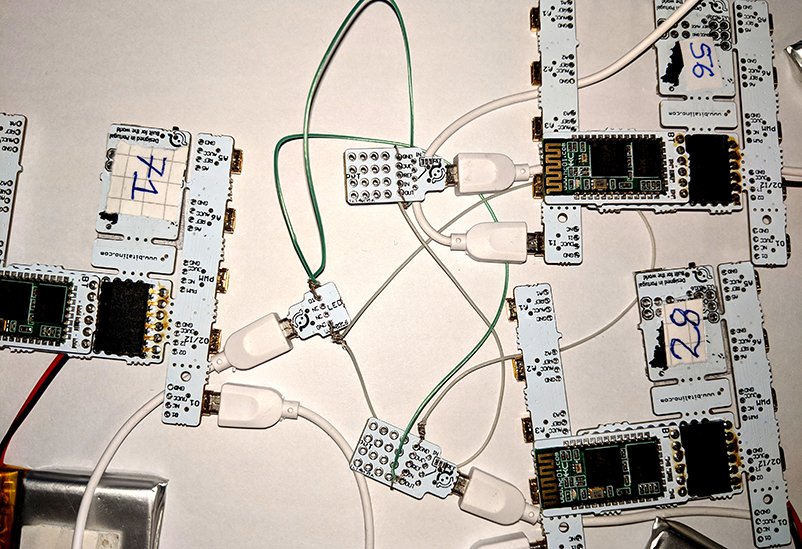
\includegraphics[width=100mm]{Figures/time_syn_bitalino.jpg}
\caption{Time synchronization of BITalino in master-slave configuration.}
\label{fig:time_sync_bitalino}
\end{figure}
\subsection{Manual Denoising}
\label{sec:denoising}
While recording with BITalino, sometimes a static noise due to electrostatic fields is generated in both ECG and EDA. The EDA recording with noise is visualized in the OpenSignals software is shown in Figure \ref{fig:eda_noisy}. We found that grounding IN+ port as shown in Figure \ref{fig:eda_denoising} denoised bot ECG and EDA signals. The denoised signal is shown in Figure \ref{fig:eda_nonnoisy}.


\begin{figure}
\centering
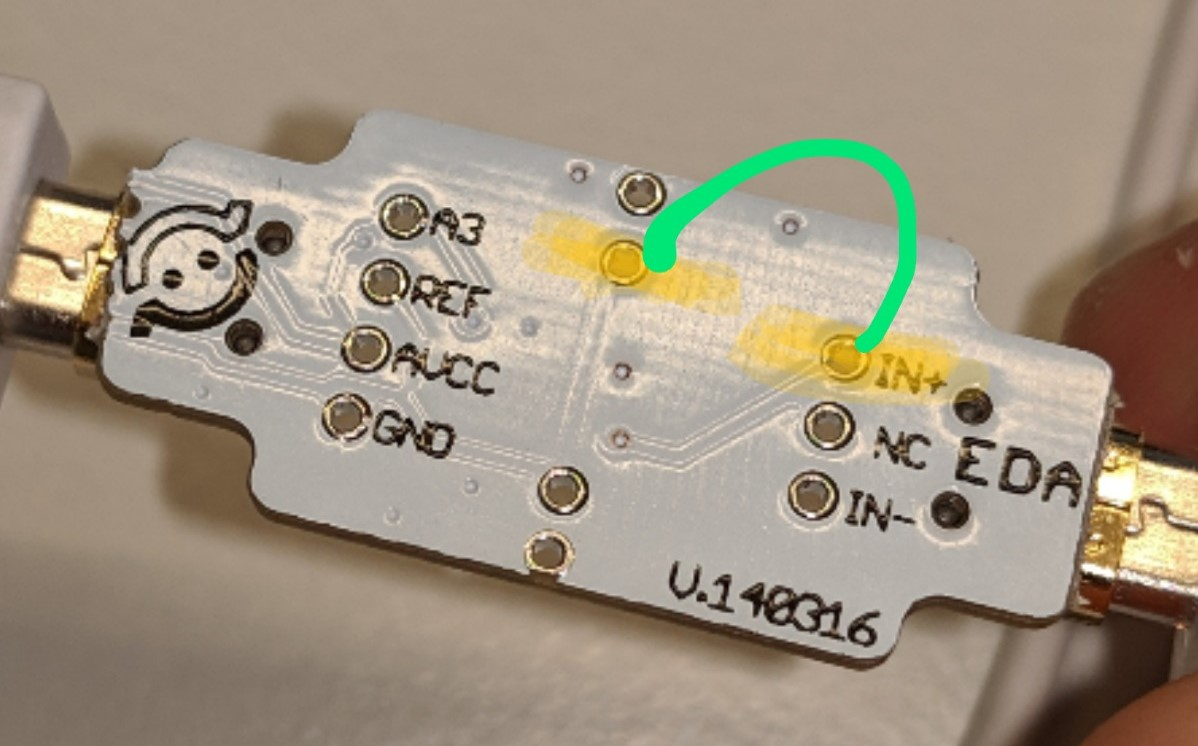
\includegraphics[width=100mm]{Figures/eda_denoising.jpeg}
\caption{Manual Denoising using EDA Sensor.}
\label{fig:eda_denoising}
\end{figure}

\begin{figure}
\centering
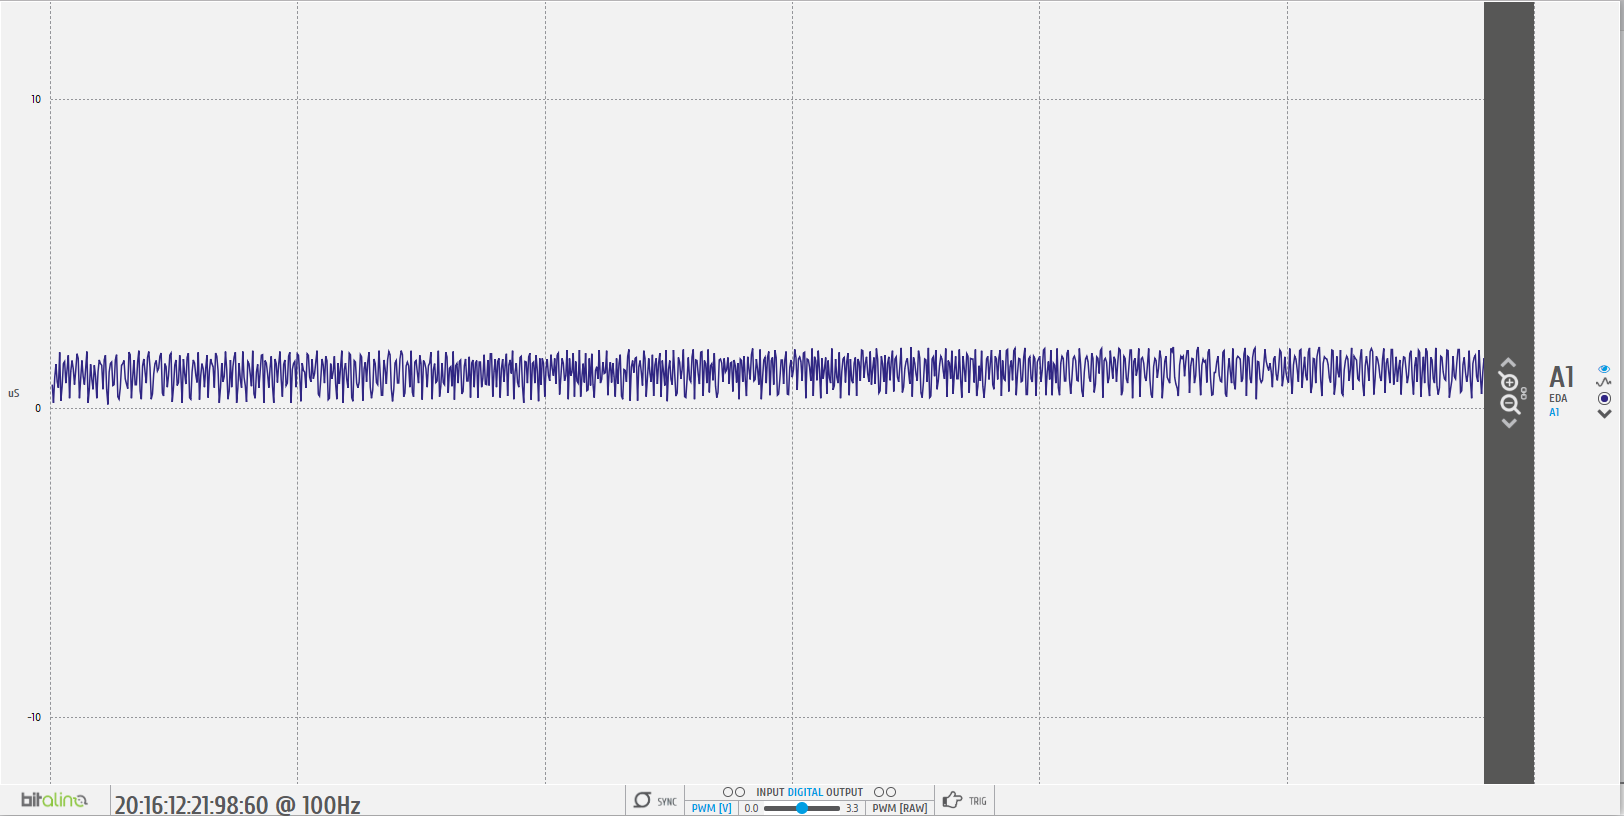
\includegraphics[width=130mm]{Figures/eda_noisy.PNG}
\caption{Noisy EDA Signal visualized in OpenSignals software.}
\label{fig:eda_noisy}
\end{figure}

\begin{figure}
\centering
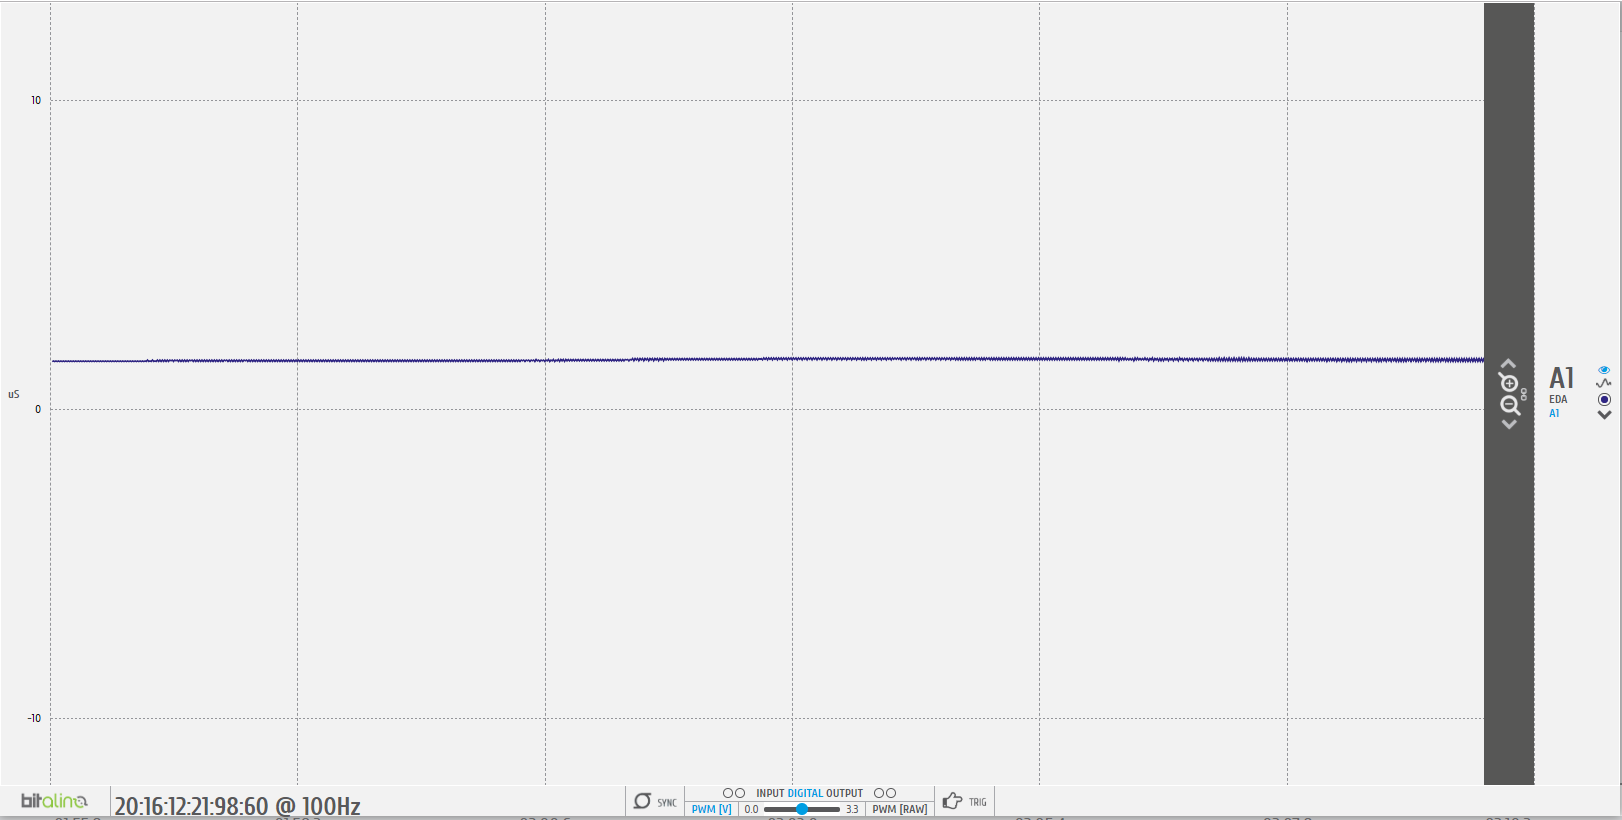
\includegraphics[width=130mm]{Figures/eda_nonnoisy.PNG}
\caption{Denoised EDA Signal visualized in OpenSignals software.}
\label{fig:eda_nonnoisy}
\end{figure}

\subsection{Web Application}
\label{sec:custom_int}
The key requirements of our experiment were: 
\begin{itemize}
    \item Accurately collect the data from multiple BITalino devices.
    \item Tag the data with synchronization information by time log of switch bit (0 or 1) for output of master device and input of slave device.
    \item Log times of when the movie started and ended, and pseudonyms of the subjects. We hence designed a web application in a client-server architecture.
\end{itemize}
\paragraph{}
The server-side of the interface shown in figure \ref{fig:bitalino_cc} is designed for the device management and playback control of the movies. The interface initiates the connection with the BITalino devices. The interface also enables the channels to be tagged with the pseudonyms of the subjects which are then written to a file. When the recording is started the server-side program reads the data from the devices in a loop and writes it to their respective files.
\paragraph{}
The second feature on the server-side enables playback control of movies on the client-side using WebSockets. The server-side interface allows playing and pausing the movie on the client-side, a browser window displayed on the projector on which movies are played. Each of these actions then creates a log file with a time stamp of the action performed along with the movie name.
\begin{figure}
\centering
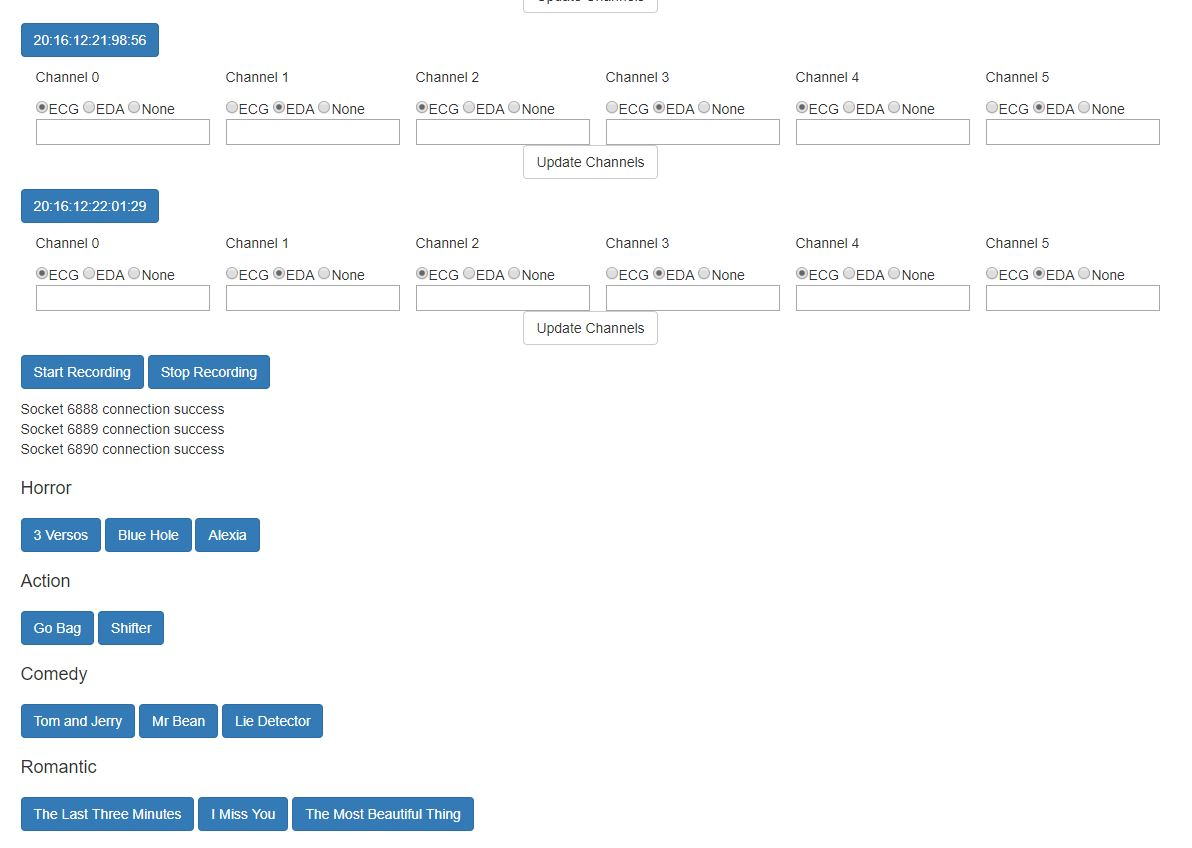
\includegraphics[width=140mm]{bitalino_interface.JPG}
\caption{BITalino Control Center.}
\label{fig:bitalino_cc}
\end{figure}

\section{Experimental Setup}
As we have discussed in Chapter \ref{sec:emo_rec}, Mood Induction Procedures (MIP) have been widely been used by scientists to understand the relation between what we see, what we hear and what we feel. Studies have shown that the range of emotions can be elicited by movies \cite{gross_emotion_1995}. As we have discussed in Chapter \ref{chapter:Terminology}, the Autonomic Nervous System is affected by the emotions and thus reflected with changes in ECG and EDA. As discussed in \ref{sec:the_methodology}, our objective in the thesis is to find a pattern in subject independent features in the ECG and the EDA recorded during a movie is being watched by the subject. With this pattern classification we can identify the movie subject is watching given their ECG and EDA data which in future might be easily acquired by fitness trackers. 

\subsection{Movie Selection} Eliciting emotional reactions from users is a difficult task. Thus selecting effective material for eliciting stimuli is crucial \cite{koelstra_deap:_2012}. We took into consideration 16 movies with an objective of short-listing 7-8 movies for the study. The main criteria for selection of movies were as follows:

\subsubsection{Run-time} The selected movies had to have a short run-time as fatigue can cause users to lose interest and hence subdue the emotions. In our initial readings we found that in a controlled setup, the users would lose interest if the movie spanned over 12-15 minutes. Thus we decided to consider only short movies in our study.
\paragraph{} We assume that the data collected for a span of under 12-15 minutes would be enough to determine the movie. Thus, this approach can also be easily adapted to a full cinema length movie, since it will contain even more information. 

\subsubsection{Genre} We considered different genres of movies for this experiment since different genres of movies induce a different array of emotions. Three from Romance, two from Horror and one each from Action, Comedy. Also, the physiological data collected could be used to identify genre instead of a specific movie.

\subsubsection{Language} All but two selected movies were in English. Two movies, from the horror genre, were in Spanish. However, both the movies had English sub-titles. The advantage of including movies of different language might help us to nullify influence of language and allowed us to include broader range of participants. Meanwhile, we also run at a risk of results being affected due to variation of data for people who do not have good proficiency in the language spoken in the movie. 
\subsubsection{Emotion Elicitation} We conducted several initial tests with our family and friends, recording their ECG and EDA to find out which movies would show greater fluctuation in the physiological readings and were interesting for the subjects.

\paragraph{} After considering all these factors we selected 7 movies for our study. The list of the movies, their genre and their run-time has been summarized in Table \ref{tab:shortlist_movies}.

\begin{center}
\begin{tabular}{ |c|c|c| }
\hline
\textbf{Movie} & \textbf{Genre} & \textbf{Run-time (mm:ss)} \\
\hline
\hline
3 Versos & Horror & 13:00 \\
\hline
Alexia & Horror & 08:55 \\
\hline
Go Bag & Action & 08:55 \\
\hline
The Lie Detector & Comedy & 03:13 \\
\hline
The Last Three Minutes & Romance & 05:19 \\
\hline
I Miss You & Romance & 06:42 \\
\hline
The Most Beautiful Thing & Romance & 10:43 \\
\hline
\end{tabular}
\captionof{table}{Short list of the movies selected for the study.}
\label{tab:shortlist_movies}
\end{center}

\subsection{Procedure}
\label{sec:procedure}
The subjects were invited to voluntarily participate in the study for compensation of 10 Euros. About 3-12 subjects participated per session. There were 13 sessions of the study conducted and 72 subject's ECG and EDA data was collected. In each session, all the subjects were asked to watch 4-5 randomly chosen movies from the list of 7 movies shown in the table \ref{tab:shortlist_movies}. Each session of the study lasted approximately 45-55 minutes.
\paragraph{}
The subjects were asked to be seated in the lecture hall at the University. The subjects were then introduced to the study procedure and were provided with the consent form. The consent form is attached in the appendix \ref{appendix_consent}.
\paragraph{}
Subjects were then asked to fill the initial questionnaire with details regarding their gender, age, language proficiency, nationality etc. The subjects were then asked to wear the AgCl electrodes as shown in the Figure \ref{fig:ecg_lead_placement} for ECG recording and Figure \ref{fig:eda_lead_placement} for EDA recording.
\paragraph{}
Thereafter, the recording of the physiological signals was initialized and lights were turned down. Subjects were asked to relax for two minutes to normalize their physiological state. At the end of two minutes, the first movie was premiered on the projector screen. After the movie ended the lights were turned on and the subjects were asked to fill the questionnaire based on the Positive and Negative Affect Schedule (PANAS) scale \cite{panas_crocker:1997} asking how much they liked the movie and emotions they felt while watching the movie. Subsequently, the rest of the movies selected for the session were played.

\subsection{Ethical Board Review}
Keeping in mind the privacy of the subjects undergoing the study. We made sure we did not collect data in any form or manner with which the subject’s identity can be revealed. We thus use pseudonyms for the subjects while collecting the data with incremental numbers, for example, Person\_1, Person\_2...
\paragraph{}
We tried to choose the audio-visual content which would not create any short-term or long-term psychological effect for the subjects. To make sure our experiment was within the ethical boundaries, we submitted our research project for review to Ethical Review Board, Department of Computer Sciences, Universit{\"a}t des Saarlandes. The board reviewed our research project and came to the conclusion that there are no ethical concerns regarding the implementation of the research project.
\paragraph{}
We further took consent from each subject by introducing them to the study procedure and its purpose. The subjects were made aware of the risks and discomforts that may occur during the study and had the right to withdraw from the study at any point and time. The consent form is attached in the appendix \ref{appendix_quest}.